\chapter{Introduzione}

Come sappiamo, tutto il sistema della crittografia a chiave
pubblica\footnote{Vedi \cite{wiki:crittografia}.} si basa sull'uso di una chiave
che ha una parte pubblica, da divulgare il più possibile, e una parte privata,
che va tenuta rigorosamente in un luogo sicuro. Qualora avessimo il dubbio che
le chiavi private possano essere in mani altrui, saremmo obbligati a generare un
nuovo mazzo di chiavi, con tutto quello che ne comporta (revoca delle chiavi,
perdita del lavoro fatto per il \emph{Web of
Trust}\footnote{\cite{wiki:webtrust}.}, perdita delle firme apposte sulla nostra
chiave).

Con questa guida vedremo come:

\begin{enumerate}
  \item \emph{generare} in un luogo abbastanza sicuro il nostro mazzo di chiavi
  personale;
  \item \emph{proteggere} le chiavi private in modo da usarle ogni giorno in un
 modo abbastanza sicuro.
\end{enumerate}

Generalmente un mazzo di chiavi personale è composto in modo predefinito da:

\begin{enumerate}
  \item una \emph{chiave master (o principale)} per la firma e la
  certificazione;
  \item una \emph{sottochiave} per la cifratura.
\end{enumerate}

Noi, invece, per elevare la sicurezza del nostro portachiavi spingeremo al
massimo il concetto delle sottochiavi. La struttura del nostro portachiavi
personale, infatti, sarà il seguente:

\begin{itemize}
  \item \emph{Chiave master (o principale) per sola certificazione di chiavi
  altrui} con dimensione 4096 bit e scadenza dopo 3 anni;
  \begin{itemize}
    \item \emph{Sottochiave per firma} con dimensione 2048 bit e scadenza dopo 1
    anno;
    \item \emph{Sottochiave per cifratura} con dimensione 2048 bit e scadenza
    dopo 1 anno;
    \item \emph{Sottochiave per autenticazione} con dimensione 2048 bit e
    scadenza dopo 1 anno.
  \end{itemize}
\end{itemize}

Avremo quindi \emph{una chiave distinta per ogni operazione}.

La chiave più importante è la \emph{chiave master}. Questa chiave è talmente
importante che, qualora fosse stata compromessa, ci costringerebbe a revocare
l'intero mazzo di chiavi e a generarne di nuove. Per questo motivo la terremo in
cassaforte, separata dal resto del mazzo di chiavi. Visto che la terremo
separata dal resto, la abiliteremo solo per scopi che non sono quotidiani, ma
periodici (come ad esempio il rinnovo della validità delle chiavi) o per
occasioni speciali (come ad esempio un \emph{Key signing
party}\footnote{\cite{wiki:ksp}.}). Lo scopo della chiave master sarà quello di
certificare chiavi altrui ed, essendo la chiave principale, di effettuare
operazioni di manutenzione del nostro mazzo di chiavi (estensione validità,
aggiunta di nomi utente, ecc.).

Le \emph{sottochiavi}, invece, saranno utilizzate quotidianamente. Le
sottochiavi hanno la caratteristica che possono esistere nel portachiavi di
GnuPG anche senza la presenza della chiave principale. Per questo motivo, dopo
aver fatto un sicuro backup, elimineremo dal portachiavi la chiave principale,
lasciando solo le sottochiavi. Le sottochiavi, per loro natura, potrebbero anche
essere compromesse (cosa che non dobbiamo permettere mai e, a tal scopo, vedremo
come proteggerle), ma questo non invaliderebbe l'intero mazzo di chiavi: qualora
una sottochiave fosse compromessa, potremmo revocarla e crearne un'altra per lo
stesso scopo. Le sottochiavi potrebbero anche scadere e, qualora non volessimo
rinnovarle, potremmo generarne di nuove. Oppure potremmo generare una
sottochiave per un evento particolare (un convegno o altro), che ha quindi una
durata limitata (un mese, un anno) e lasciarla scadere dopo la fine dell'evento.

\begin{wrapfloat}{figure}{r}{0pt}
    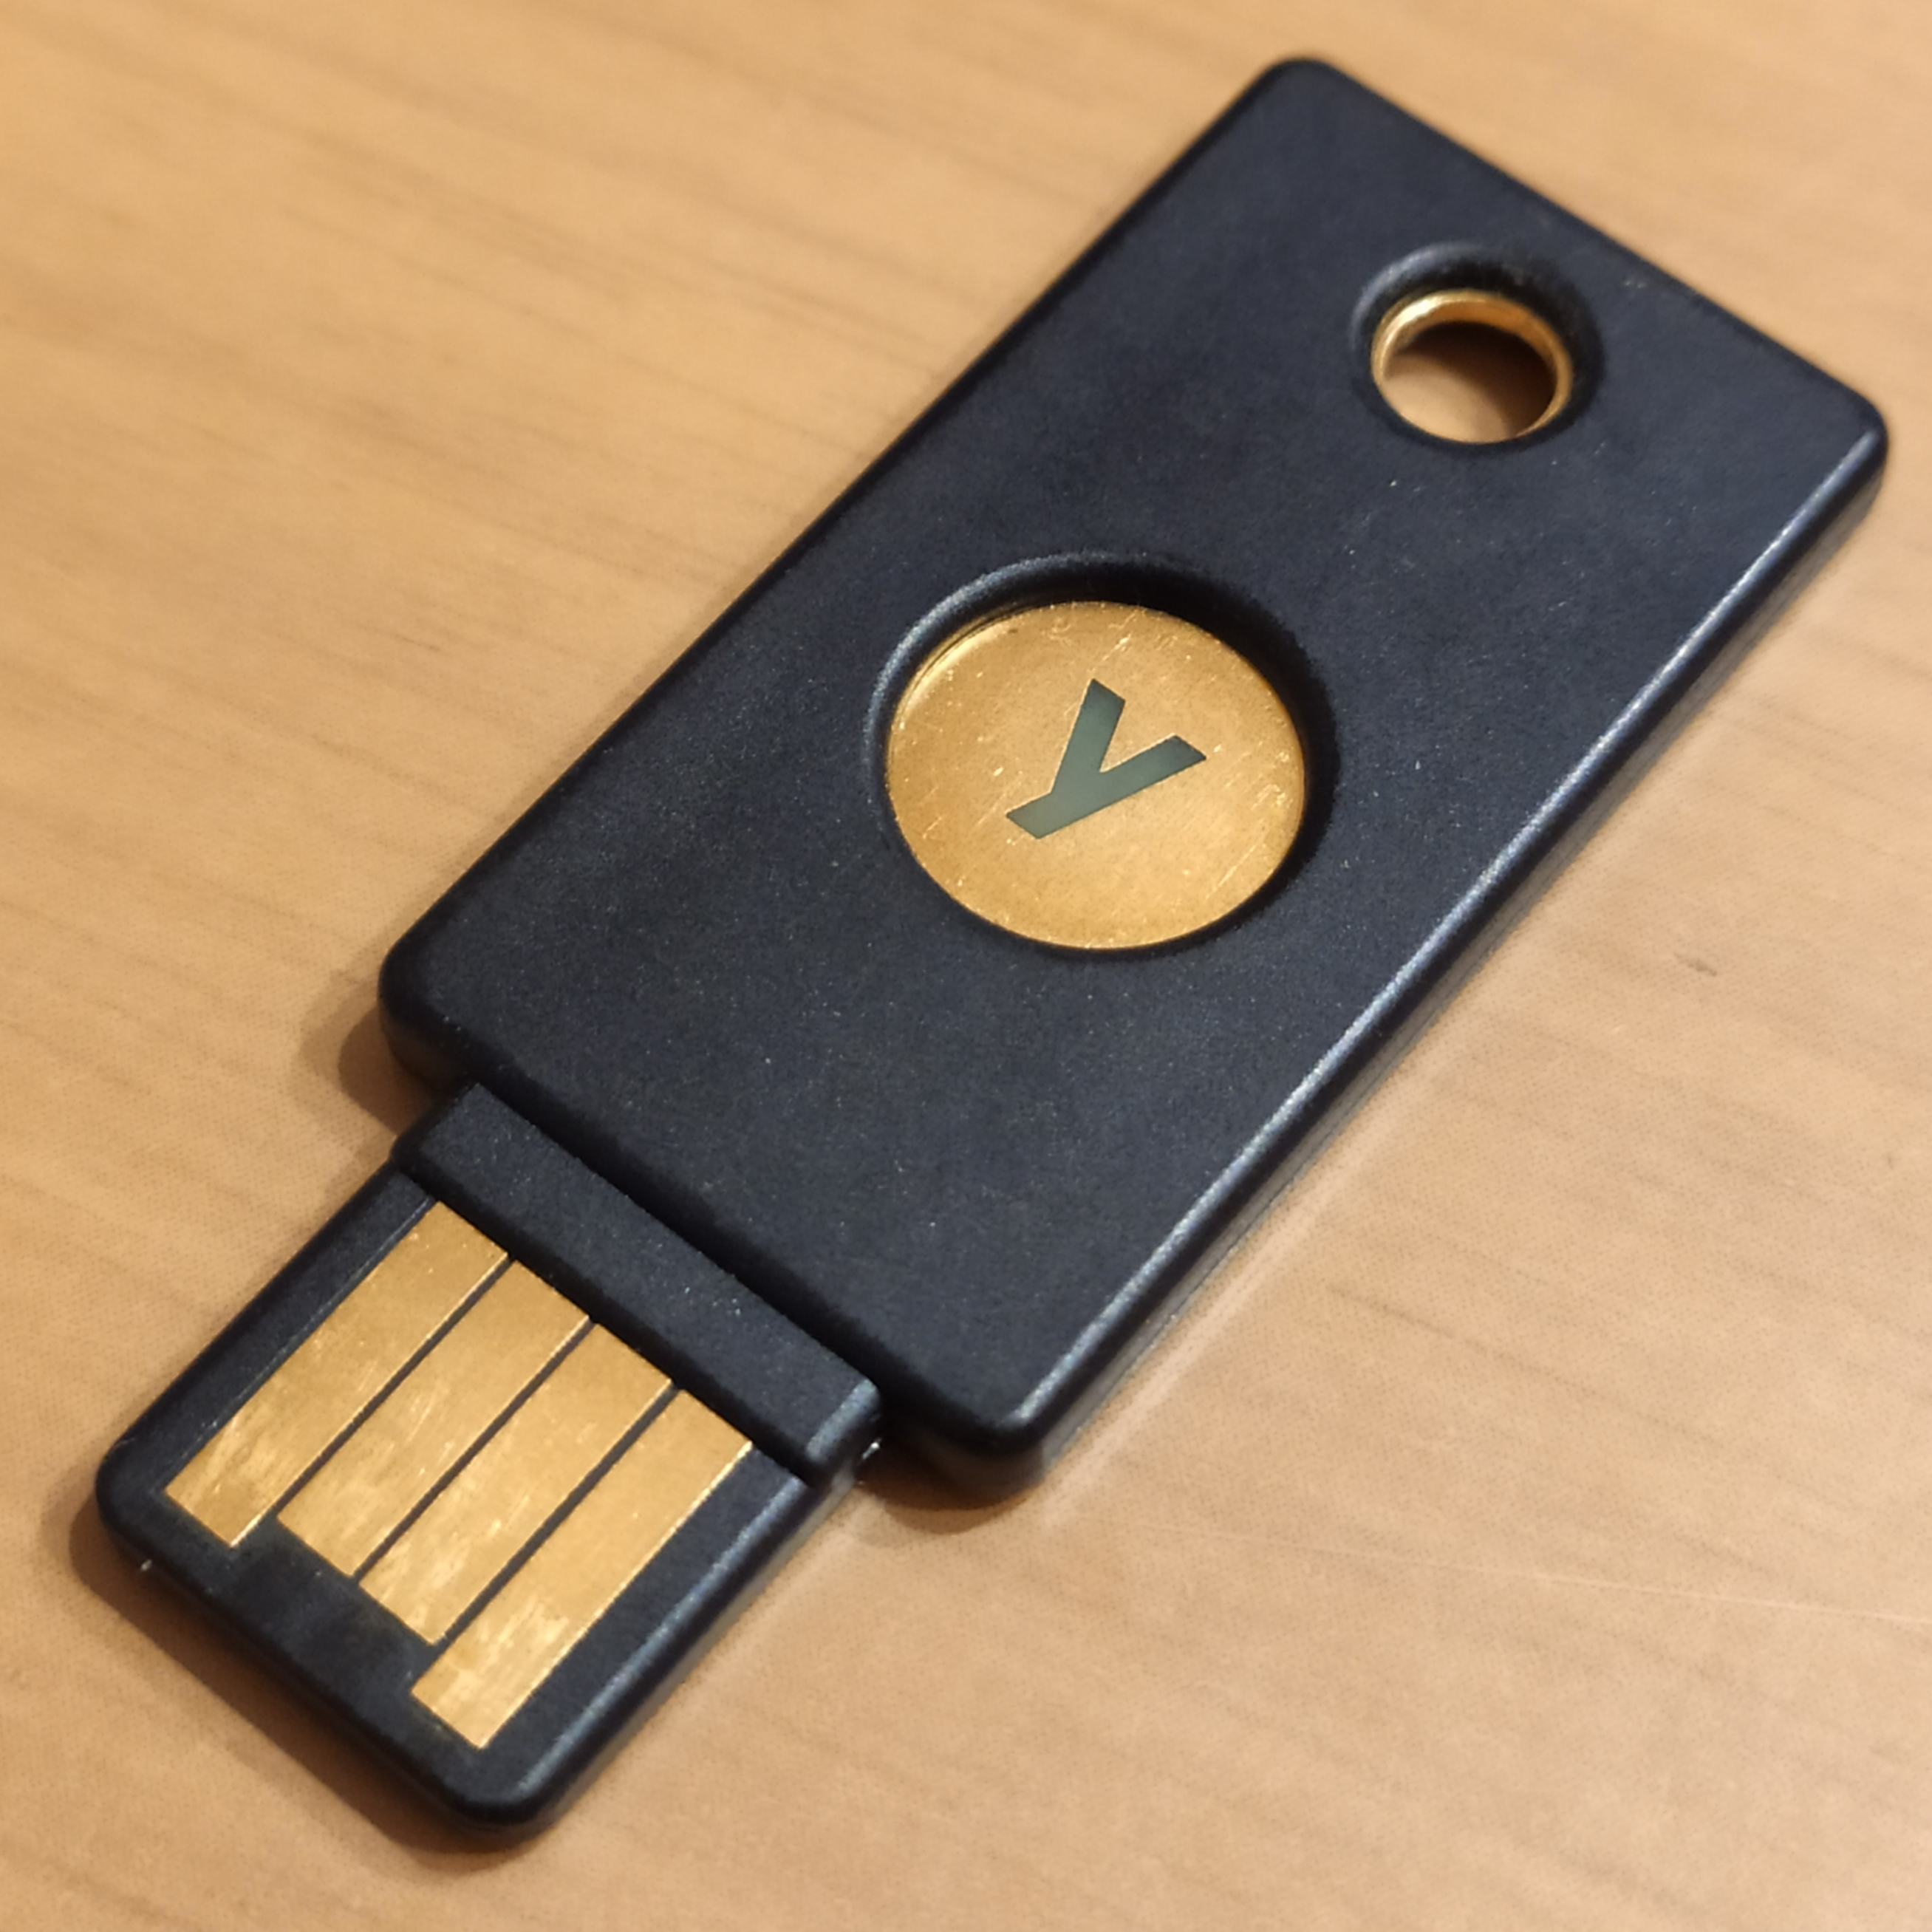
\includegraphics[width=0.33\textwidth]{yubikey4}
    \caption{La YubiKey 4 di Yubico.}
    \label{fig:yubikey4}
\end{wrapfloat}

Per proteggere le nostre sottochiavi, le sposteremo su \emph{un token
\textsc{usb} come la YubiKey}.\footnote{\url{https://www.yubico.com/}.} Si
tratta di token praticamente indistruttibili, che rendono l'uso della firma
digitale, la cifratura e l'autenticazione su sistemi (come \textsc{ssh}) molto
comodi, dato che basterà usare un \textsc{pin} numerico al posto della
passphrase. Io uso la YubiKey
4,\footnote{\url{https://www.yubico.com/product/yubikey-4-series/\#yubikey-4}}
come da figura \ref{fig:yubikey4}. I token come YubiKey hanno il pregio che non
permettono l'esportazione delle chiavi lì conservate; questo significa che posso
usare le mie chiavi anche in un ambiente poco sicuro come un Internet Point, un
\textsc{pc} condiviso, ecc., senza il timore che le chiavi private possano
essere copiate da qualche parte a mia insaputa. Quand'anche fosse stato
intercettato il \textsc{pin} da un keylogger o da un malware, la passphrase è
ancora al sicuro, ed eventualmente posso cambiare il \textsc{pin}. Il fatto che
le sottochiavi, una volta trasferite, non possano essere esportate dalla
YubiKey, ci forzerà a effettuare il backup del nostro mazzo di chiavi prima del
trasferimento, ma questo aspetto lo vedremo al momento opportuno.

Alla fine della guida avremo quindi la seguente situazione:

\begin{enumerate}
  \item \emph{la chiave principale} sarà rimossa dal portachiavi sul disco e trasferita
  in un luogo sicuro;
  \item \emph{le sottochiavi} risiederanno sulla YubiKey.
\end{enumerate}

Nel nostro disco fisso non avremo quindi nessuna chiave privata. Potremmo anche
perdere il nostro \textsc{pc} o potrebbero anche rubarcelo, ma il nostro mazzo
di chiavi sarà sempre al sicuro. Potremmo anche perdere la nostra YubiKey, ma
essa contiene solo le sottochiavi che, come abbiamo visto, possiamo revocare con
la chiave principale (che sta in cassaforte) e ricrearne di nuovi. Quando sarà
necessario effettuare un'operazione speciale, come ad esempio apporre la nostra
firma su chiavi altrui o aggiungere/eliminare una sottochiave o una UserID,
importeremo la chiave principale nel nostro portachiavi, effettueremo
l'operazione necessaria e infine la rimuoveremo di nuovo.\bigskip

\noindent Un ultimo punto prima di passare alla pratica. Il motivo di avere una
scadenza sulle chiavi è un ulteriore sicurezza per noi. Immaginiamo il caso in
cui dovessimo perdere il controllo del nostro mazzo di chiavi, compresa la
chiave principale, e non avessimo più a disposizione nemmeno il certificato di
revoca. In questo caso la scadenza sarà una garanzia per noi che a un certo
punto le chiavi scadranno in modo naturale. Per i tempi di scadenza ognuno può
scegliere quello che più ritenga opportuno, ma 3 anni per la principale e 1 anno
per le sottochiavi dovrebbe essere un buon compromesso tra la seccatura di dover
manutenzionare il portachiavi e il tempo di scadenza naturale dopo eventuale
compromissione.\bigskip

\noindent Questa guida può essere seguita in modo modulare:

\begin{itemize}
  \item si può scegliere di mantenere tutte le chiavi sul proprio disco fisso,
  seguendo solo la parte sulla generazione sicura delle chiavi;
  \item si può scegliere di spostare in un luogo sicuro la chiave principale dal
  resto del proprio mazzo di chiavi, mantenendo nel disco fisso solo le
  sottochiavi;
  \item si può scegliere di spostare le sottochiavi in un token \textsc{usb}
  come la YubiKey, mantenendo la chiave principale nel disco fisso;
  \item si può scegliere di spostare le sottochiavi in un token \textsc{usb}
  come la YubiKey e di spostare la chiave principale in un luogo sicuro, non
  lasciando nessuna chiave privata nel disco fisso.
\end{itemize}\bigskip

\noindent Una nota prima di cominciare. Lungo la guida i vari comandi da
terminale useranno \textsc{id} di chiave, keygrip, percorsi nel disco fisso e
quant'altro che fanno riferimento a quanto eseguito per scrivere la guida. Ciò
significa che dovrete sostituire gli \textsc{id} di chiave, i keygrip, i
percorsi e quant'altro con quelli vostri. Ad esempio, in un comando come questo:

\begin{lstlisting}
gpg --with-keygrip --list-key 0x9F676B5A4B6E6777
\end{lstlisting}

\noindent dovrete sostituire \texttt{0x9F676B5A4B6E6777} con l'\textsc{id}
corretto della vostra chiave.

Inoltre, il percorso \texttt{/home/user} va modificato inserendo il nome utente
corretto al posto di \texttt{user}.
